\documentclass{article}
\usepackage[utf8]{inputenc}
\usepackage{graphicx}
\usepackage{hyperref}

\title{Research Methodology UE18CS400SG \\ Unit 1}
\author{Aditeya Baral}
\date{January 2022}

\begin{document}

\maketitle

\section{Meaning of Research}

\begin{itemize}
    \item Research (re -- search, search -- examine carefully and probe) is a careful and systematic study in some field of knowledge, undertaken to establish facts or principles.
    \item Organized and systematic way of finding answers to questions.
    \item A careful investigation or inquiry specially through search for new
facts in any branch of knowledge.
    \item \textbf{Redman and Mory} -- \textit{"Systematized effort to gain new knowledge."}
    \item \textbf{Clifford Woody} --
    \begin{itemize}
        \item Defining and redefining problems
        \item Formulating hypothesis or suggested solutions
        \item Collecting, organising and evaluating data
        \item Making deductions and reaching conclusions
        \item Carefully testing the conclusions to determine whether they fit the
formulating hypothesis.
    \end{itemize}
    \item \textbf{D. Slesinger and M. Stephenson in the Encyclopaedia of Social
Sciences} -- \textit{“The manipulation of things, concepts or symbols for the purpose of generalising to extend, correct or verify knowledge, whether that
knowledge aids in construction of theory or in the practice of an art.”}
\end{itemize}

\subsection{Objectives of Research}

\begin{itemize}
    \item To gain familiarity with a phenomenon or to achieve new insights into it
    \item To portray accurately the characteristics of a particular individual,
situation or a group
    \item To determine the frequency with which something occurs or with which
it is associated with something else
    \item To test a hypothesis of a causal relationship between variables
\end{itemize}

\subsection{Motivation for Research}

\begin{itemize}
    \item Research Degree
    \item Challenge in solving unsolved problems
    \item Joy in doing creative work
    \item Service to society
    \item Respectability
\end{itemize}

\subsection{Types of Research}

\begin{enumerate}

    \item \textbf{Descriptive vs Analytical}
    \begin{enumerate}
        \item Descriptive -- description of state of affairs as it exists
        \item Analytical -- Use facts or information already
available and analyze these to make a critical evaluation of the material
        \item \textbf{Characteristic} -- No control over variables, only report what has happened/happening
        \item Methods involve comparative and correlation
    \end{enumerate}
    
    \item \textbf{Applied vs Fundamental}
    \begin{enumerate}
        \item Applied Research -- Focused on solving immediate problem facing a society or an industrial business organization aimed at conclusions (like health, pollution, environment, safety etc)
        \item Fundamental -- concerned with generalizations and with the formulation of a theory
    \end{enumerate}
    
    \item \textbf{Quantitative vs Qualitative}
    \begin{enumerate}
        \item Quantitative -- measurement of quantity, controlled, easy to carry out, objective, repeatable, easy to draw conclusions and decisions
        \item Qualitative -- qualitative phenomenon, discover underlying motives of behaviour, opinion research, difficult
    \end{enumerate}
    
    \item \textbf{Conceptual vs Empirical}
    \begin{enumerate}
        \item Conceptual -- related to abstract ideas or theory, used by philosophers and thinkers to develop new concepts/reinterpret existing ones
        \item Empirical -- relies on experience or observation, data based and verified by experiments, \textbf{control over variables under study}, evidence through empirical studies is considered as the most powerful support for a hypothesis 
    \end{enumerate}
    
    \item \textbf{Other types} -- one time, longitudinal, field, laboratory, simulation, clinical, diagnostic, historical etc
    
\end{enumerate}

\subsection{Research Method vs Methodology}

\begin{itemize}
    \item \textbf{Method} -- technique or method adopted to conduct research - data collection, statistical methods to establish relationship between data and variables, evaluation methods for accuracy of results
    \item \textbf{Methodology} -- Way in which research problem is solved systematically
\end{itemize}

\subsection{Research Process}

\begin{figure*}[htp]
    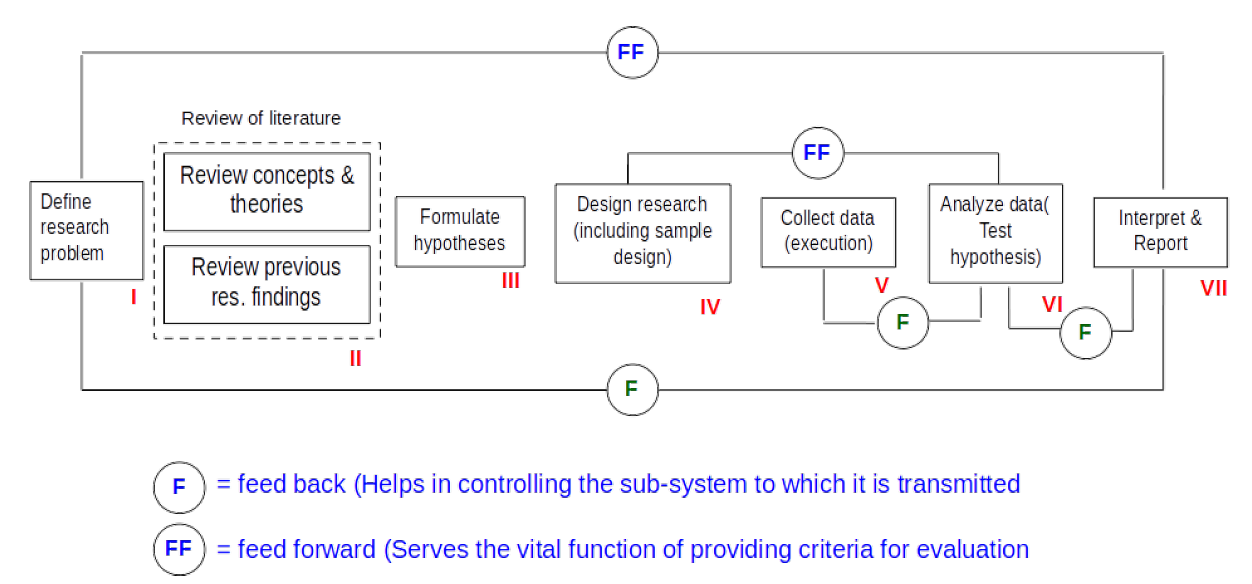
\includegraphics[width=1 \linewidth]{img/flowchart.png}
    \caption{Research Process}
    \label{fig:flowchart}
\end{figure*}

\begin{enumerate}

    \item \textbf{Formulating the research problem}
        \begin{enumerate}
            \item Understand research problem thoroughly
            \item Rephrase in meaningful terms
        \end{enumerate}
        
    \item \textbf{Extensive literature survey} -- abstracting and indexing journals, conference proceedings, reports, books, internet for earlier studies on topic
    
    \item \textbf{Developing the hypothesis}
        \begin{enumerate}
            \item \textbf{Working Hypothesis} -- temporary assumption made to draw out and test logical consequences
            \item Affect manner of conducting tests
            \item Process -- discussion with colleagues, examination of data and records, review similar studies, exploratory personal investigation like field interviews
        \end{enumerate}
    
    \item \textbf{Preparing the research design} -- concerns with how to obtain information, availability and skills of researcher and staff, time and cost factor (financial) for research

    \item \textbf{Determining sample design} -- simple random, systematic, stratified, quota, cluster, sequential etc
    
    \item \textbf{Collecting the data} -- observation, surveys, personal/telephonic interviews, questionnaires
    
    \item \textbf{Execution of the project}
    
    \item \textbf{Analysis of data} -- coding, tabulation, statistical tests and measures
    
    \item \textbf{Hypothesis Testing}
        \begin{enumerate}
            \item \textbf{Hypothesis} is a proposed explanation for a phenomenon. A hypothesis is scientific if it can be tested. Scientific hypothesis are based on previous observations that cannot be explained with available theories.
            \item Choose appropriate test like chi-square test, t-test, f-test etc based on nature of research and accept or reject hypothesis
        \end{enumerate}
    
    
    \item \textbf{Generalizations and Interpretation} -- arrive at certain generalization and interpret and explain findings based on some theory
    
    \item \textbf{Preparation of the report or Presentation of the results, i.e., formal write-up of conclusions reached}
        \begin{enumerate}
            \item Concise report with clear charts and illustrations
            \item Introduction, summary of findings, main report, conclusion
        \end{enumerate}
\end{enumerate}

\subsection{Criteria for Good Research}

\begin{itemize}
    \item Purpose should be clearly defined
    \item Procedure used should be described in sufficient detail
    \item Design of research should be carefully planned to yield result as objective
    \item Report – complete frankness, flaws in procedural design
    \item Analysis should be sufficiently adequate, method of analysis should be appropriate
    \item Conclusion should be confined to those justified by data of research
\end{itemize}

\subsection{Properties of Good Research}

\begin{itemize}
    \item \textbf{Systematic} -- structured with specific steps in sequence
    \item \textbf{Logical} -- guided by by rules of logical reasoning, logical procedure for induction and deduction
    \item \textbf{Empirical} -- related to one or more aspects of a real situation, deals with data
    \item \textbf{Replicable} -- results can be verified by replicating study, builds on sound basis of decision
\end{itemize}

\section{Literature Review}

\begin{itemize}
    \item A broad, comprehensive, in-depth, systematic, and critical
review of scholarly publications
    \item Surveys, summarizes and links together research in a given field
    \item Laborious but essential (may constitute entire project itself)
    \item Critical and effective evaluation of available literature on research topic -- overview of problem under study
    \item Leads logically to the research question
\end{itemize}

\subsection{Introduction to Literature Review}

\subsubsection{Importance of Review of Literature}

\begin{itemize}
    \item Identification, development, refinement of requirements
    \item Identification of gaps/inconsistencies
    \item Strength and weaknesses of designs/methods/instruments used in research work
    \item Development of plan -- research methodology
    \item Development of Research Hypothesis
\end{itemize}

\subsubsection{Purpose of Review of Literature}

\begin{itemize}
    \item Overview and guide to a topic
    \item Provides solid background for investigation
    \item Updated with current developments in research field
    \item Critical look at literature
    \item Demonstrates relevance of research
    \item Determines
        \begin{itemize}
            \item Research Design, method of study -- instruments, data collection and analysis
            \item Knowns and unknowns
            \item Inconsistencies and consistencies
            \item Strengths and weaknesses
            \item Unanswered questions
            \item Refinement of problem, hypothesis and justifications
        \end{itemize}
\end{itemize}

\subsubsection{Functions of Review of Literature}

Background information, establish importance, familiarity and make space for future research

\subsubsection{Goal of Review of Literature}
\begin{itemize}
    \item Demonstrate mastery over a subject
    \item Locate area of current research in present literature
\end{itemize}

\subsubsection{Sources of Review of Literature}

\begin{itemize}
    \item \textbf{Primary} -- written by person(s) who developed theory or conducted research
    \item \textbf{Secondary} -- written by person(s) except those who developed theory or conducted research. Used when primary source is unavailable or to look at the problem from different angles
\end{itemize}

Databases, journals, research reports, books, conference papers, encyclopedias, dictionaries, magazines, newspapers are sources

\subsubsection{What to look for in a Review of Literature}

\begin{itemize}
    \item Clearly defined problem
    \item Goodness of design
    \item Validity of results
    \item Flaws in logic
    \item Ignored problems
\end{itemize}

\subsection{Writing Literature Review}

\begin{enumerate}
    \item Organize Studies
    \begin{enumerate}
        \item Chronological -- publication date, trend
        \item Thematic -- based on themes
        \item Methodological -- example, qualitative vs quantitative
    \end{enumerate}
    
    \item List down
    \begin{enumerate}
        \item Facts
        \item Opinions
        \item Variables and their relationship with concepts
        \item Shortcomings and limitations in existing methods
        \item Relevance of research
        \item Suggestions for future work
    \end{enumerate}
    
    \item Start with introduction, then discussion of sources followed by conclusion with summary of findings relevant to current study
    
    \item After writing, read for coherence and check for errors in logic
\end{enumerate}

\subsubsection{Stages of Writing}
\begin{itemize}
    \item Problem formulation -- field under study, issues
    \item Literature search -- finding materials
    \item Data evaluation -- determine which literature is a significant contribution
    \item Analysis and interpretation
\end{itemize}

\subsubsection{Critiquing Criteria for reading Review of Literature}

\begin{itemize}
    \item Uncover gaps and inconsistencies
    \item Ensure relevancy of concepts and variables
    \item Reveal relevant components of study, design, strengths, weaknesses, conflicts
    \item Include concepts, data in present literature
    \item Include summary
    \item Follow a logical sequence and signify direction of research (justification of problem and leading up to hypothesis)
\end{itemize}

\subsubsection{Points to Ensure while writing Review of Literature}

\begin{itemize}
    \item Specific and succinct -- no details or in-depth analysis
    \item Selective -- important points only
    \item Focus on current work
    \item Ensure reliability of sources of evidence
    \item Reference citations to literature in bibliography
    
\end{itemize}

\subsubsection{Properties of a good Review of Literature}

\begin{itemize}
    \item Focused -- narrow topic
    \item Concise but developed (don't leave out details)
    \item Logical sequence of ideas
    \item Integrative -- similarities/difference among literature, how it contributed to topic
    \item Current -- focus on latest work
    
\end{itemize}

\section{Research Problem}

\textit{"Research Problem, in general, refers to some difficulty which a researcher experiences in the context of either a theoretical or practical situation and wants to obtain a solution for the same"}

\begin{itemize}
    \item A specific issue, difficulty, contradiction, or gap in knowledge that one must aim to address in their research
    \item Points to the need for meaningful understanding and systematic investigation
\end{itemize}

If $ I $ is the individual, $ N $ is the environment defined by $ Y_j $ uncontrolled variables, $ C $ is a course of action and $ O $ is an outcome, then a research problem exists if,

\begin{equation}
    P (O_1 | I, C_1, N) \neq P(O_1 | I, C_2, N)
\end{equation}

Different choices must have unequal probabilities for desired outcomes.

\begin{figure}
\begin{center}
    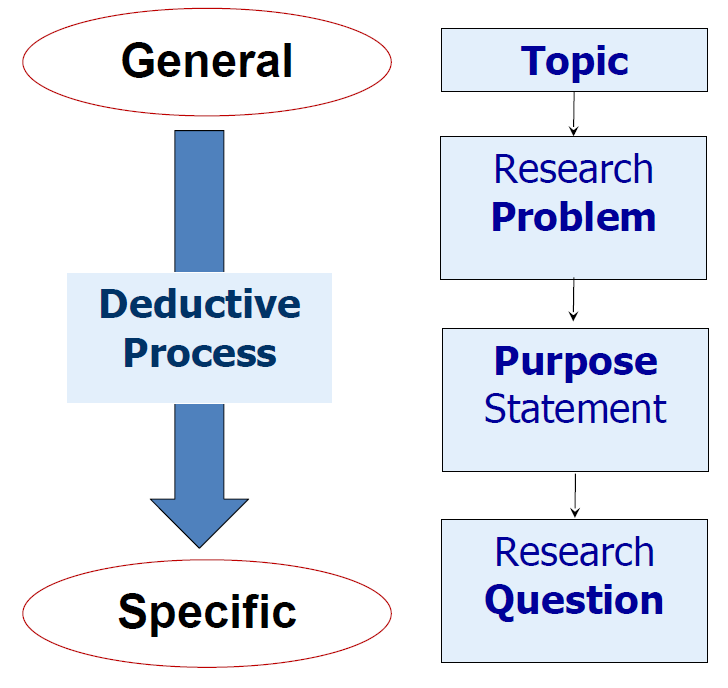
\includegraphics[scale=0.25]{img/research-problem.png}
    \caption{Refinement of Research Topic to Research Process}
    \label{fig:research-problem}
    \end{center}
\end{figure}

\subsection{Elements of Problem Statement}

\begin{itemize}
    \item Topic -- subject area
    \item Issue -- concern/problem needing solution
    \item Evidence of issue -- literature/experience
    \item Deficiencies in evidence -- what do we need to know more
    \item Remedy of deficiencies -- how the solution helps people
\end{itemize}

\subsection{Sources of Research Problems}

Experience, existing research and theories, social issues, brainstorming, intuitions, exposure to field situations and consultation with experts

\subsection{Selecting a Research Problem}

\begin{itemize}
    \item Subject is not overdone
    \item Avoid controversial subjects and vague problems
    \item Subject is familiar and feasible
    \item Must be preceded by preliminary study
\end{itemize}

\subsection{Defining a Research Problem}

\textit{"A clearly defined research problem is half solved"}

Task of defining a research problem is sequential -- state problem, resolve ambiguities, more specific formulation to make it realistic and meaningful

\begin{enumerate}
    \item State the problem in a general way
    \item Understand nature of problem
    \item Survey literature
    \item Develop ideas through discussion
    \item Rephrase research problem
    \item Clearly define terms and phrases
    \item State basic assumptions and postulates
    \item State criteria for selection of problem
    \item State suitability of time period and data sources
    \item State scope of investigation
\end{enumerate}

\subsection{Properties of a well defined Research Problem}

\begin{itemize}
    \item Meaningful
    \item Paves way for development of working hypothesis
    \item Helps solve the problem
\end{itemize}

\end{document}
